\chapter{Proxy and VPN Clients}

\section{Comparing Clients}
Traditional clients like v2rayN are powerful but require manual rule curation. Smart Relay aims to keep the power while automating decisions with AI.

\section{Control vs Data Plane}
The control plane decides routes and pushes configs to the data plane engines (xray, sing-box). Smart Relay ships adapters to bridge the decision layer to the engines.

\section{Example Deployment Topology}
\begin{figure}[h]
    \centering
    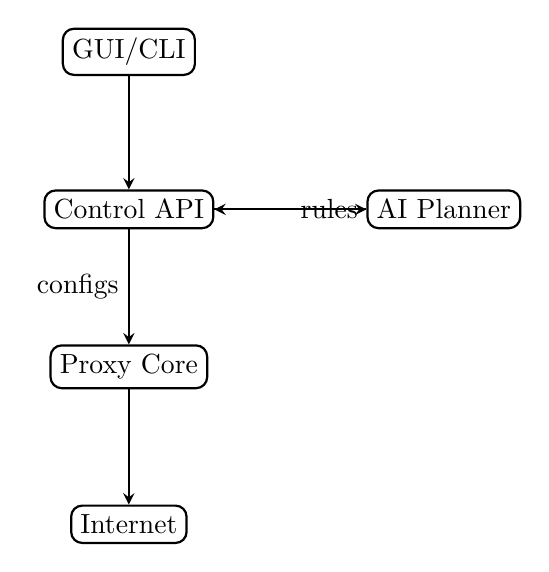
\begin{tikzpicture}[node distance=2cm,>=stealth,thick]
        \node (ui) [draw, rounded corners] {GUI/CLI};
        \node (api) [draw, rounded corners, below of=ui] {Control API};
        \node (ai) [draw, rounded corners, right of=api, xshift=2cm] {AI Planner};
        \node (core) [draw, rounded corners, below of=api] {Proxy Core};
        \node (internet) [draw, rounded corners, below of=core] {Internet};
        \draw[->] (ui) -- (api);
        \draw[->] (api) -- (ai);
        \draw[->] (ai) -- node[right]{rules} (api);
        \draw[->] (api) -- node[left]{configs} (core);
        \draw[->] (core) -- (internet);
    \end{tikzpicture}
    \caption{Control plane automates decisions; data plane forwards traffic.}
\end{figure}

\section{Key Features for a Modern Client}
\begin{itemize}
    \item Health-aware routing based on live probes.
    \item Zero-trust posture with minimal local secrets.
    \item First-class API for GUI, mobile, and scripting.
\end{itemize}

\section{Routing Strategies You Should Know}
\begin{itemize}
    \item \textbf{Geo-biasing}: steer video to low-latency regions, bulk downloads to cheapest egress.
    \item \textbf{Fail-open vs fail-closed}: pick policy per app; corporate traffic likely fail-closed.
    \item \textbf{Split tunneling}: only proxy destinations that need it; measure MTU/PMTU to avoid fragmentation.
    \item \textbf{Multi-hop}: optional double proxy for censorship-heavy regions; watch compounded latency.
\end{itemize}

\section{Core Integration Notes}
Start with a thin adapter that writes xray/sing-box JSON, validates it, then hot-reloads. Keep adapters isolated so UI/API never depends on a specific core schema.

\section{Suggested Checklists}
\begin{itemize}
    \item Preflight: DNS reachability, clock sync, certificate presence.
    \item Runtime: probe endpoints every N seconds, update scores, adjust weights.
    \item Postmortem: capture last applied config, probe logs, and AI rationale.
\end{itemize}

